\documentclass[11pt]{article}
\usepackage[margin=1in]{geometry}
\usepackage{booktabs}
\usepackage{graphicx}
\usepackage{amsmath}
\usepackage{caption}
\usepackage[hidelinks]{hyperref}
\captionsetup{font=small,labelfont=bf}
\setlength{\parskip}{4pt}
\setlength{\parindent}{0pt}

\newcommand{\dsd}{DS\textsubscript{disrupted}}
\newcommand{\dsh}{DS\textsubscript{healthy}}
\newcommand{\hct}{HC\textsubscript{trust}}
\newcommand{\hce}{HC\textsubscript{equal}}

\title{\textbf{Understanding the Fixed-Routing World:}\\
\large the allocation bound, the residual cost, and the system's dynamics\\
\normalsize (follow-up to the routing study; same scenario, no new regime)}
\author{Aidan Hansen}
\date{June 10, 2026}

\begin{document}
\maketitle

\section*{Summary}
The routing study showed that fixing the order-routing rules removes 67--91\% of the
disruption cost and restores a 1.000 fill rate. Before changing anything about the scenario,
we finished understanding it: (E1) \emph{is there any value left in the distributor's
allocation lever?} (E2) \emph{what is the remaining 1.21M cost made of?} (E3) \emph{how do
the dynamics actually play out?} Findings: the allocation channel is worth \textbf{at most
10--12\%}, the entire upside is captured by a \emph{trivial static-priority rule} (at a
fairness cost), and plausible-looking dynamic rules make things up to \textbf{56\% worse};
the residual cost is mostly \emph{bookkeeping at the dead factory} (41\%) plus the
unavoidable $\sim$10-period redirection transient, not a patient-service problem; and the
one genuine physical inefficiency left --- a post-recovery inventory glut that our own
stale-order write-off \emph{doubles} --- is a small, fixable design artifact. Conclusion:
\textbf{in this scenario there is no meaningful room left for learned policies}; what remains
are two small deterministic refinements.

\section{Setup}

\begin{table}[h]
\centering\small
\caption{All experiments run on the routing-fixed (rung c) baseline of the routing study:
both HCs trust-split with trust$^4$ weights ($\delta'=0.3$), stale-order write-off
($k=5$), base-stock ordering everywhere. Reporting seeds 11--30, paired; phases pre 60--109 /
during 110--157 / post 158--300; system-level cost (all six agents).}
\begin{tabular}{lp{10.6cm}}
\toprule
\textbf{Experiment} & \textbf{Design} \\
\midrule
E1 allocation bound & DS allocation family \{proportional, equal, priority-HC1,
priority-HC2, backlog-priority, serve-captive\}, applied at both DSs, closed loop. No tuned
parameters. Max-over-family spread bounds the channel. Gate: the new code path under
`proportional' reproduces rung c \emph{bit-for-bit} (60 columns $\times$ 300 periods). \\
E2 residual decomposition & Rung-c's 1.21M during+post cost, decomposed by agent $\times$
phase $\times$ (holding $\mid$ backlog); glut quantified. Pure analysis of existing logs;
totals cross-check against the routing study (pass). \\
E3 dynamics anatomy & Period-by-period trust, order routing, receipts, on-order ledger
vs.\ counted, up-to targets, dead-factory queue. Pure analysis of existing logs. \\
\bottomrule
\end{tabular}
\end{table}

\section{E1 --- The allocation bound}

\begin{table}[h]
\centering\small
\caption{Allocation family on the rung-c baseline. dp-cost = during+post system cost
(urgent0; SEs $\le$ 0.4\% of means). Lost patients from the urgent20 config (episode total).
Total units shipped are identical across rules --- every difference is a closed-loop
trust-feedback effect.}
\begin{tabular}{lrrr}
\toprule
\textbf{Allocation rule} & \textbf{dp-cost} & \textbf{vs.\ proportional} & \textbf{Lost patients} \\
\midrule
priority-HC1 / -HC2 (static) & \textbf{1{,}060k} & $\mathbf{-12.4\%}$ & \textbf{445} \\
proportional (= rung c) & 1{,}210k & --- & 510 \\
equal & 1{,}209k & $-0.0\%$ & 509 \\
serve-captive & 1{,}517k & $+25\%$ & 603 \\
backlog-priority & 1{,}881k & $+56\%$ & 795 \\
\bottomrule
\end{tabular}
\end{table}

Three readings. \textbf{(i) The channel is second-order}: 10--12\% at best, against routing's
67--91\%. \textbf{(ii) The upside is trivial to capture and symmetric}: strict static priority
wins, and it does not matter which HC is prioritized --- what wins is \emph{consistency}
(serve one customer fully, keep its delivery/trust loop clean) rather than any clever
targeting. The gain costs fairness: the non-prioritized HC's during fill drops to 0.957 vs.\
0.981 (urgent20); proportional and equal are fairness-neutral. If fairness is a hard
constraint, the channel's usable upside is $\approx$ zero. \textbf{(iii) The downside is
$5\times$ the upside}: backlog-priority --- the ``obvious'' smart rule --- alternates failures
across both HCs, keeps both trust loops degraded, and lands 56\% \emph{worse} with more lost
patients. For the eventual DRL comparison this bounds Mechanism 3 (allocation intelligence)
tightly and asymmetrically: a learner exploring this space has little to win and much to lose.

\section{E2 --- What the remaining 1.21M is made of}

\begin{table}[h]
\centering\small
\caption{Rung-c during+post system cost by agent (urgent0, mean over seeds).}
\begin{tabular}{lrl}
\toprule
\textbf{Agent} & \textbf{Cost} & \textbf{Dominant component} \\
\midrule
MN\textsubscript{disrupted} & 498k (41\%) & orders queued at the shut factory (backlog cost, up to 48 periods) \\
\dsd{} & 345k (29\%) & early orders + the $\sim$10-period redirection transient \\
\dsh{} & 122k (10\%) & the absorption transient \\
HCs (both) & 183k (15\%) & brief service dip (during) + recovery holding (post) \\
MN\textsubscript{healthy} & 61k (5\%) & carrying the surge \\
\bottomrule
\end{tabular}
\end{table}

None of this is a during-disruption service problem (fill is 1.000). Two observations for
discussion. \textbf{The glut is real and partly self-inflicted}: post-disruption system
inventory peaks at 3{,}930 vs.\ a pre-disruption mean of 332 --- \emph{double} the baseline's
glut (2{,}051) --- because the write-off lets \hce{} re-order from the healthy chain while the
written-off stale orders still deliver late. The cost (post holding 135k vs.\ 107k baseline)
is $\sim$20$\times$ smaller than the backlog cost the write-off saves, but a recovery-aware
refinement could keep the savings without the glut. \textbf{A modeling question for the
advisor}: 41\% of the residual is backlog cost accruing on undeliverable orders queued at a
shut factory --- an accounting convention, not a physical loss. Under a patient-facing lens
the true residual is roughly half the headline number.

\begin{figure}[h]
\centering
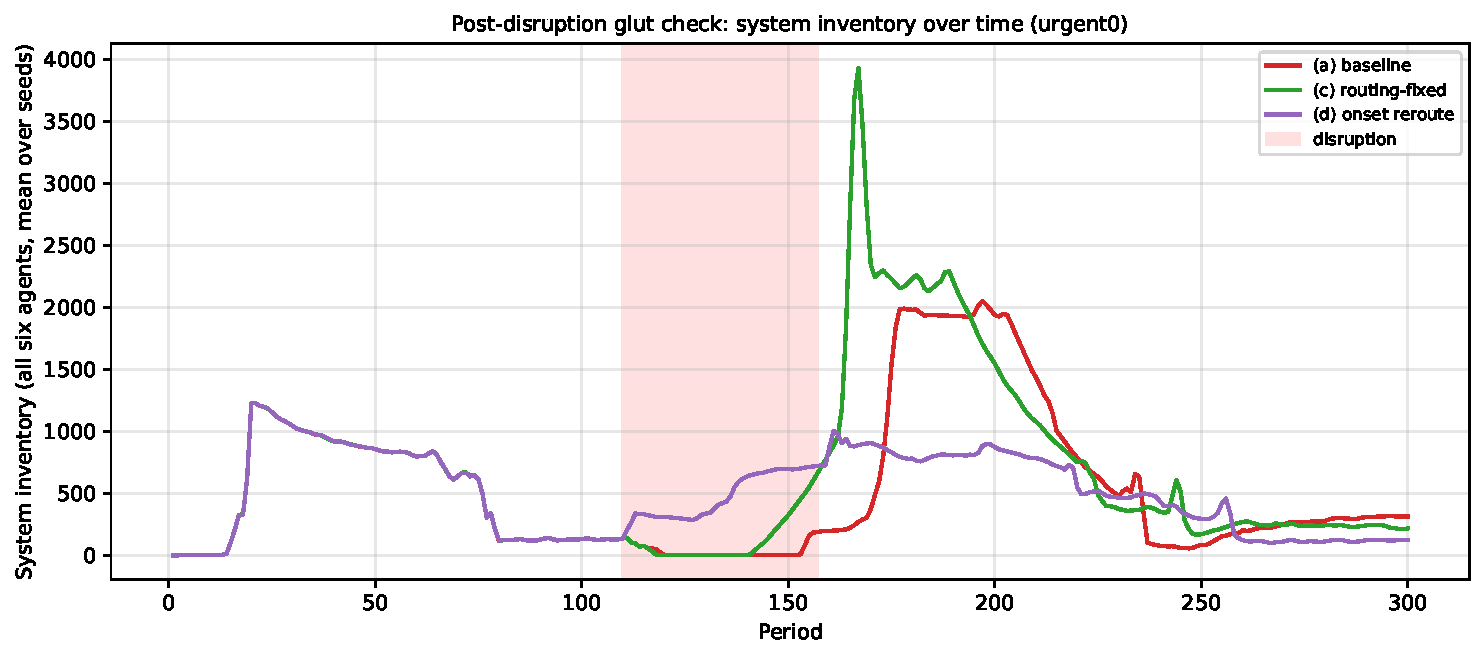
\includegraphics[width=0.95\textwidth]{../results/figures/glut_trajectories.pdf}
\caption{System inventory over time. The rung-c glut (green, peak 3{,}930) is double the
baseline's (red) and almost six times the oracle-reroute rung's (purple) --- the price of the
accounting-only write-off, visible and fixable.}
\end{figure}

\section{E3 --- How the fixed-routing world actually moves}

\begin{figure}[h]
\centering
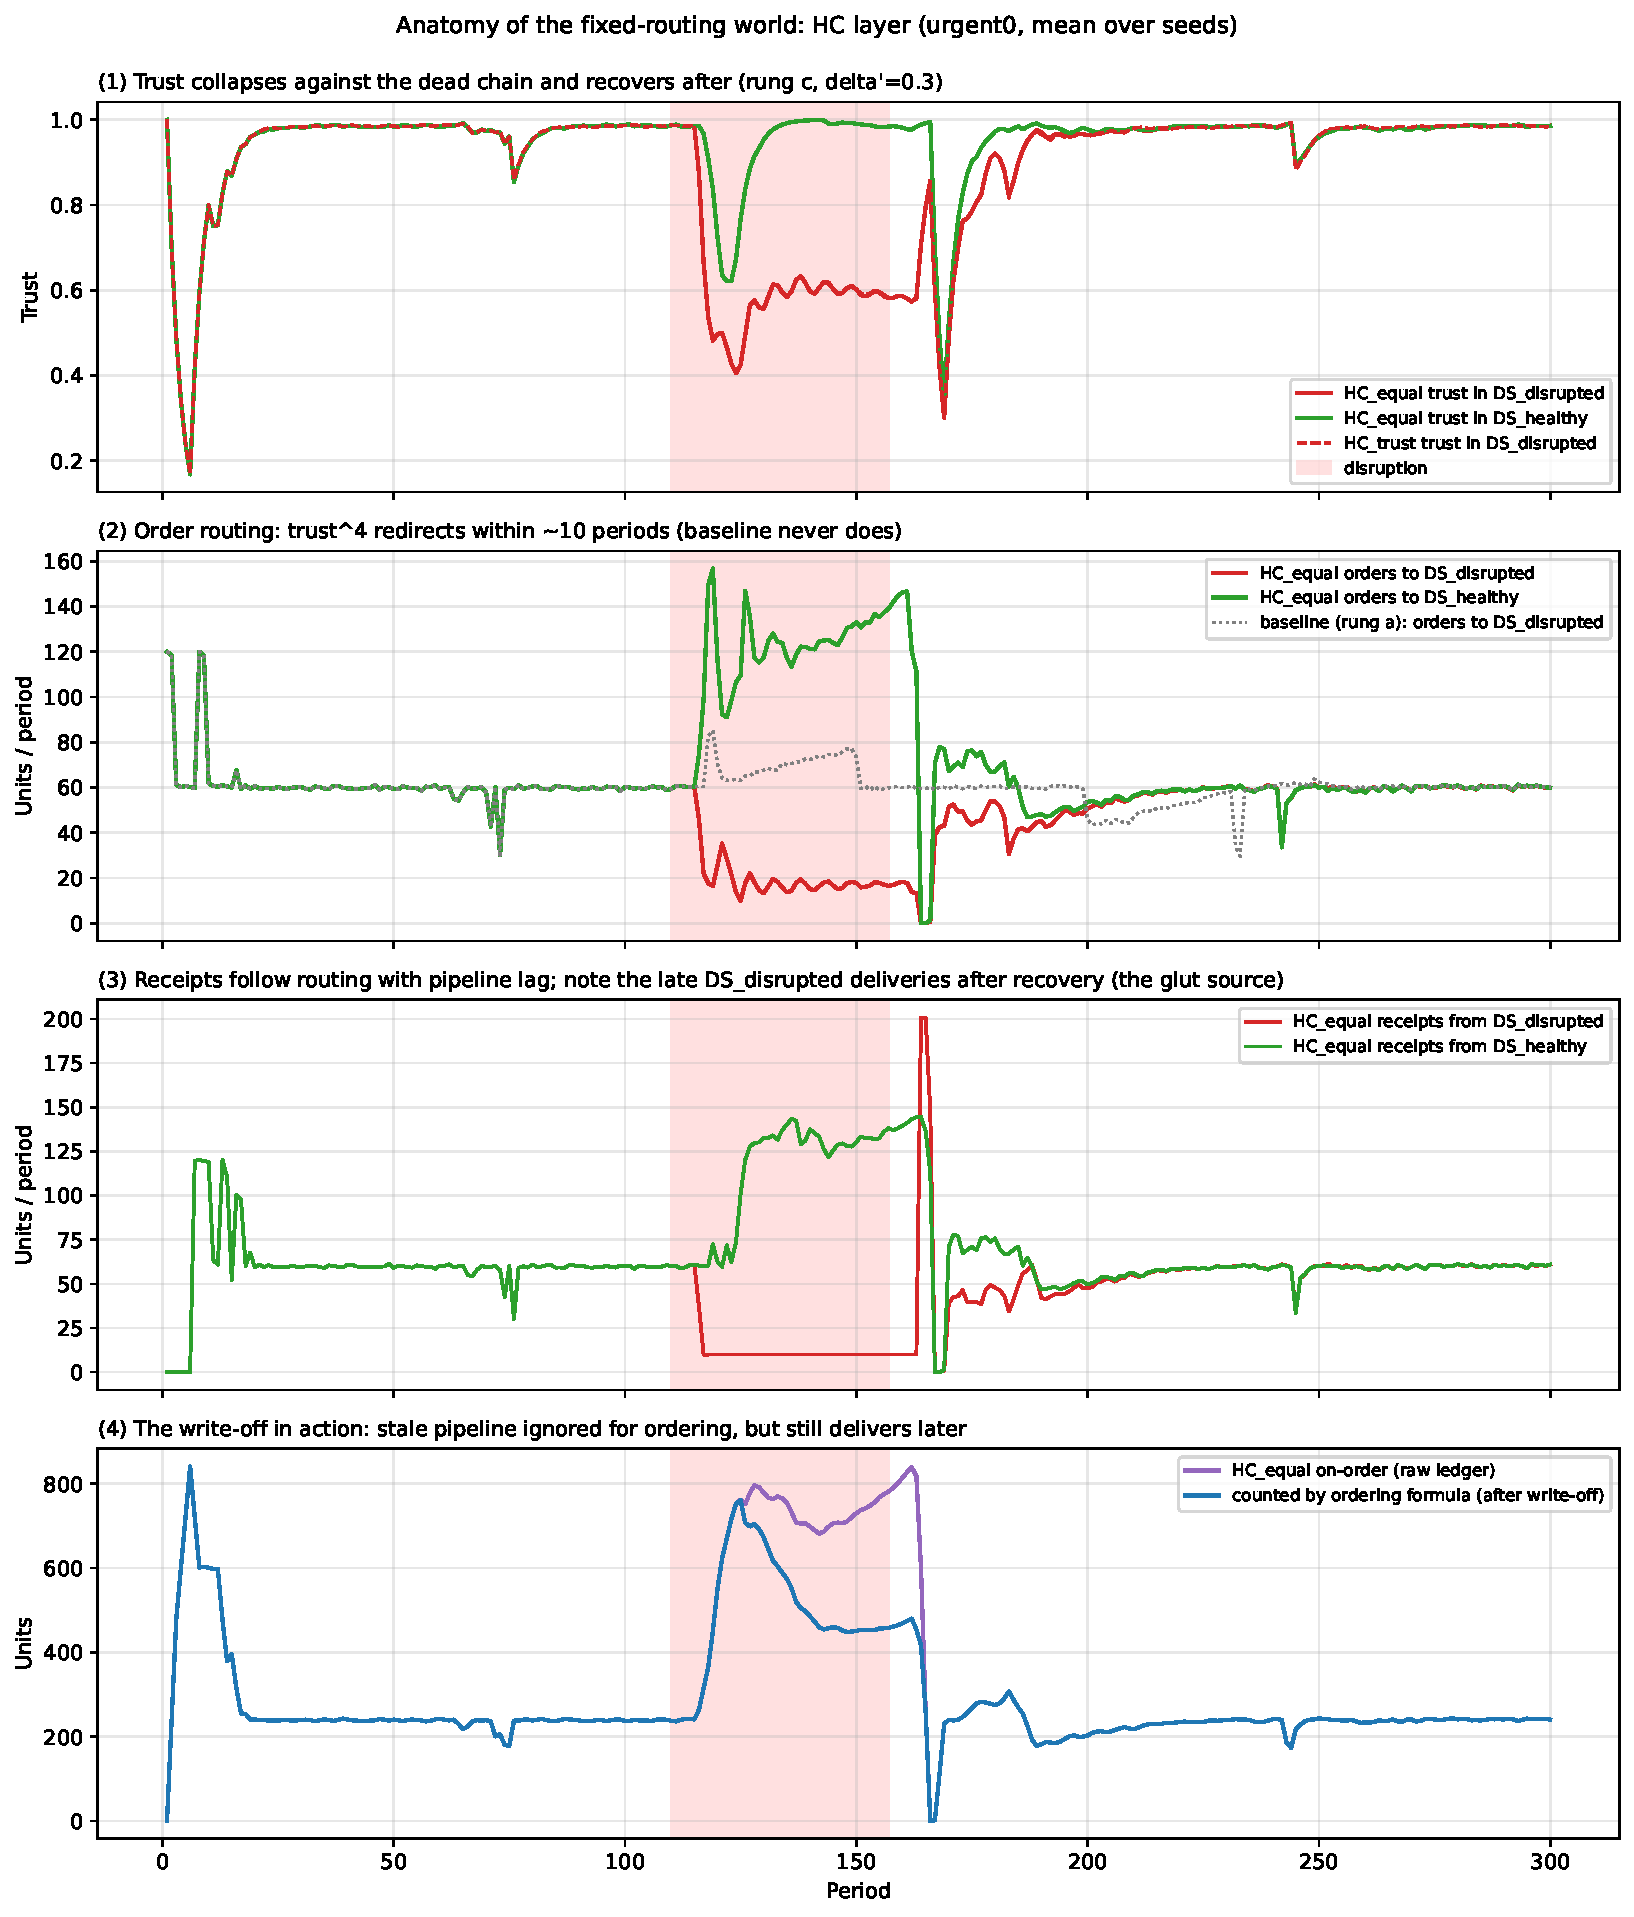
\includegraphics[width=0.88\textwidth]{../results/figures/anatomy_hc_layer.pdf}
\caption{HC layer. (1) Trust collapses to $\sim$0.55 in $\sim$10 periods (the EMA floor ---
the trickle keeps delivering, so trust never reaches 0) and recovers $\sim$20 periods after
the disruption. (2) Orders follow trust; the baseline (dotted) never moves. (3) Receipts
follow orders with pipeline lag; the recovery-time spike of late deliveries from the dead
chain is the glut arriving. (4) The write-off: the raw on-order ledger climbs to $\sim$800
while the ordering formula counts only $\sim$450 --- the ignored gap is what frees \hce{}
to re-order from the healthy chain.}
\end{figure}

\begin{figure}[h]
\centering
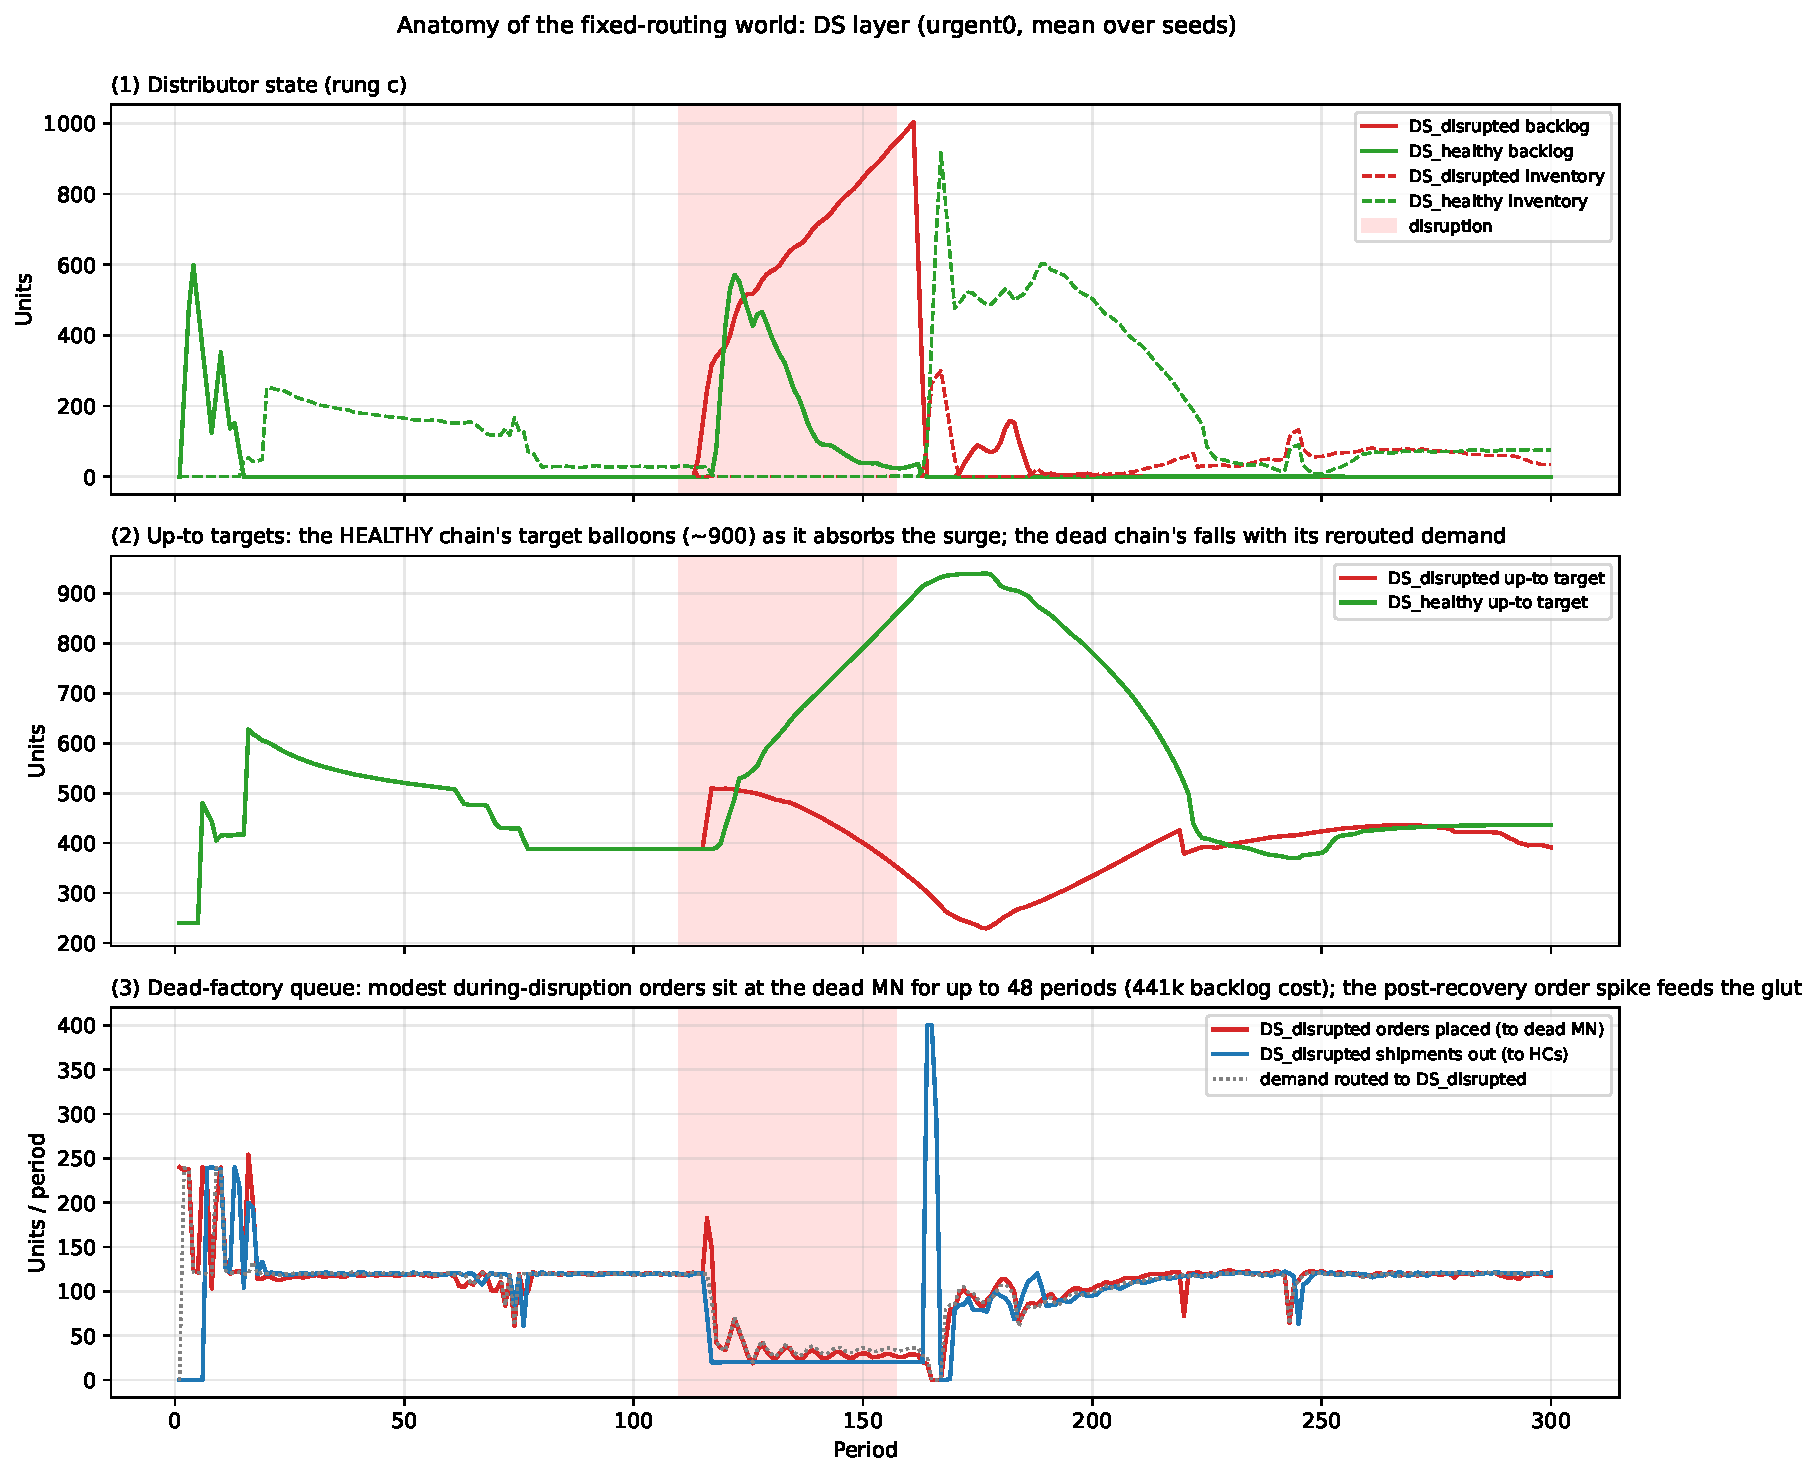
\includegraphics[width=0.88\textwidth]{../results/figures/anatomy_ds_layer.pdf}
\caption{DS layer. (1) \dsd{}'s backlog peaks at $\sim$1{,}000 (vs.\ 4{,}100 baseline);
\dsh{} absorbs with a brief $\sim$570 transient. (2) A counterintuitive finding: the
\emph{healthy} chain's up-to target balloons to $\sim$900 (its lead time stretches under the
surge) while the dead chain's target \emph{falls} with its rerouted demand. (3) \dsd{}'s
during-disruption orders are modest, but they queue at the shut factory for the whole window
(the 441k); the post-recovery catch-up spike feeds the glut.}
\end{figure}

\clearpage
\section{What we learned, and next steps}

\textbf{What we learned.}
\begin{enumerate}
\item \textbf{The scenario is essentially solved by routing.} With routing fixed, fill rate
is 1.000; no remaining cost is a patient-service problem.
\item \textbf{The allocation channel --- the last DS-level lever, and the last place a DRL
contribution could hide in this scenario --- is bounded at 10--12\%}, fully captured by a
trivial static rule, bought at a fairness cost, with a $5\times$ asymmetric downside for
getting it wrong. There is no meaningful room left for learned policies here.
\item \textbf{The residual cost is mostly accounting} (41\% dead-factory queue bookkeeping)
plus an unavoidable $\sim$10-period transient; the one physical inefficiency (the glut) is a
fixable artifact of our own write-off design.
\item \textbf{Two dynamics surprises} worth carrying: the healthy chain's up-to target is the
one that balloons (not the dead chain's), and consistency beats cleverness in allocation
because of the trust feedback loop.
\end{enumerate}

\textbf{Next steps (in order).}
\begin{enumerate}
\item \textbf{Recovery-aware write-off refinement} (deterministic, small): suppress
re-ordering as written-off pipeline approaches delivery --- removes the glut, closes the main
self-inflicted cost.
\item \textbf{Recompute the buffer sweep and clairvoyant ceiling on the rung-c baseline} ---
the gating step before any value-decomposition number goes in a paper.
\item \textbf{Write up the simple scenario completely} (routing study + this study). Only
then consider robustness regimes (severity/duration sweeps), introduced because the write-up
demands generality --- not to give tools a job.
\item \textbf{When the corrected DRL arrives}: evaluate it against the new compound simple
baseline --- rung-c routing + static-priority allocation. The bar: beat 1.06M during+post
cost (urgent0) / 445 lost patients (urgent20) without losing fairness.
\end{enumerate}

\end{document}
